% compile with: lualatex -shell-escape filename.tex
\documentclass[svgnames, tikz]{standalone}
\directlua{luatexbase.add_to_callback(
  "wrapup_run",
  function() os.execute("pdf2svg \jobname.pdf \jobname.svg") print("Converted to SVG.") end,
  "final callback to convert pdf file")}

\usetikzlibrary{positioning}

\tikzset{box1/.style={draw, minimum size=0.9cm}}
\tikzset{box2/.style={draw, minimum height=0.9cm, minimum width=1.9cm}}
\tikzset{box3/.style={draw, minimum height=0.9cm, minimum width=3.9cm}}
\tikzset{box4/.style={draw, minimum height=0.9cm, minimum width=7.9cm}}
\tikzset{box5/.style={draw, minimum height=0.9cm, minimum width=15.9cm}}
\tikzset{label/.style={color=black!50, font=\tiny}}

\begin{document}
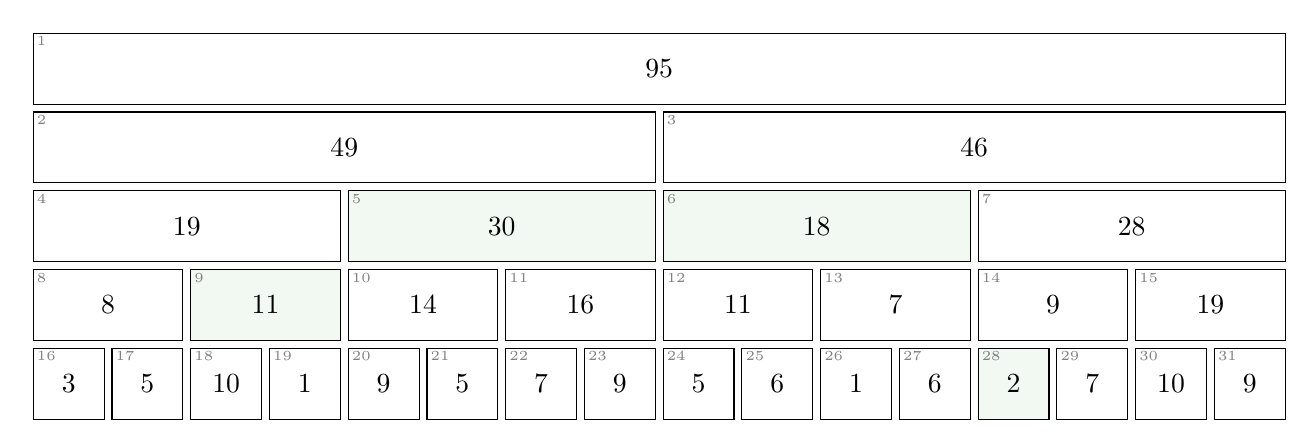
\begin{tikzpicture}

  \node [box5] at ( 7.5, 4) (node1)  {95};

  \node [box4] at ( 3.5, 3) (node2)  {49};
  \node [box4] at (11.5, 3) (node3)  {46};

  \node [box3] at ( 1.5, 2) (node4)  {19};
  \node [box3, fill=Green!5] at ( 5.5, 2) (node5)  {30};
  \node [box3, fill=Green!5] at ( 9.5, 2) (node6)  {18};
  \node [box3] at (13.5, 2) (node7)  {28};

  \node [box2] at ( 0.5, 1) (node8)  { 8};
  \node [box2, fill=Green!5] at ( 2.5, 1) (node9)  {11};
  \node [box2] at ( 4.5, 1) (node10) {14};
  \node [box2] at ( 6.5, 1) (node11) {16};
  \node [box2] at ( 8.5, 1) (node12) {11};
  \node [box2] at (10.5, 1) (node13) { 7};
  \node [box2] at (12.5, 1) (node14) { 9};
  \node [box2] at (14.5, 1) (node15) {19};

  \node [box1] at ( 0, 0) (node16) { 3};
  \node [box1] at ( 1, 0) (node17) { 5};
  \node [box1] at ( 2, 0) (node18) {10};
  \node [box1] at ( 3, 0) (node19) { 1};
  \node [box1] at ( 4, 0) (node20) { 9};
  \node [box1] at ( 5, 0) (node21) { 5};
  \node [box1] at ( 6, 0) (node22) { 7};
  \node [box1] at ( 7, 0) (node23) { 9};
  \node [box1] at ( 8, 0) (node24) { 5};
  \node [box1] at ( 9, 0) (node25) { 6};
  \node [box1] at (10, 0) (node26) { 1};
  \node [box1] at (11, 0) (node27) { 6};
  \node [box1, fill=Green!5] at (12, 0) (node28) { 2};
  \node [box1] at (13, 0) (node29) { 7};
  \node [box1] at (14, 0) (node30) {10};
  \node [box1] at (15, 0) (node31) { 9};

  \foreach \i in {1,...,31} {
%    \node [label, above left=-0.3 and -0.4 of node\i] {\i};
    \node [label, below right=-0.1 of node\i.north west] {\i};
  }

\end{tikzpicture}
\end{document}
